\section{Extra}

\subsection{Hanoi Tornyai}
\begin{frame}{Hanoi Tornyai}
    \begin{center}
        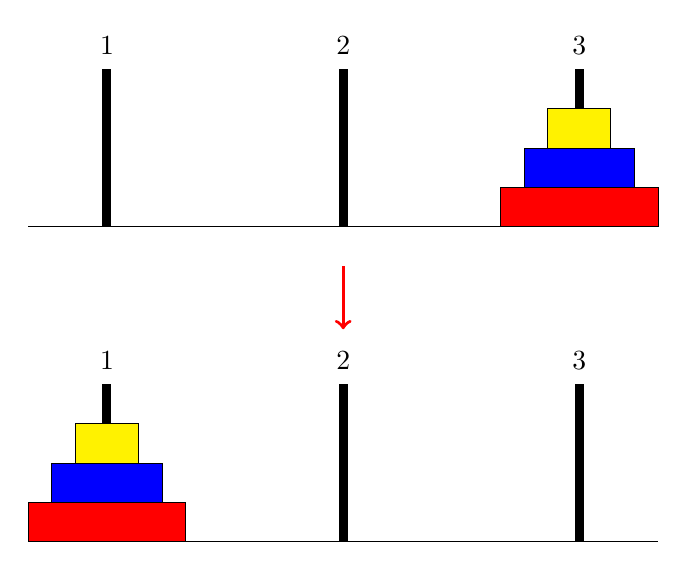
\begin{tikzpicture}
            \draw (-4,2.3) node{1};
            \draw (-1,2.3) node{2};
            \draw (2,2.3) node{3};
        
            \draw (-5,0) -- (3,0);
            \filldraw[fill=black] (-4.05,2) rectangle (-3.95,0);
            \filldraw[fill=black] (-1.05,2) rectangle (-0.95,0);
            \filldraw[fill=black] (1.95,0) rectangle (2.05,2);
            
            \filldraw[fill=red] (1,0) rectangle (3,0.5);
            \filldraw[fill=blue] (1.3,0.5) rectangle (2.7,1);
            \filldraw[fill=yellow] (1.6,1) rectangle (2.4,1.5);
            
            \draw[->,very thick,red] (-1,-0.5) -- (-1,-1.3);
        
            \draw (-4,-1.7) node{1};
            \draw (-1,-1.7) node{2};
            \draw (2,-1.7) node{3};
        
            \draw (-5,-4) -- (3,-4);
            \filldraw[fill=black] (-4.05,-4) rectangle (-3.95,-2);
            \filldraw[fill=black] (-1.05,-4) rectangle (-0.95,-2);
            \filldraw[fill=black] (1.95,-4) rectangle (2.05,-2);
        
            \filldraw[fill=red] (-5,-4) rectangle (-3,-3.5);
            \filldraw[fill=blue] (-4.7,-3.5) rectangle (-3.3,-3);
            \filldraw[fill=yellow] (-4.4,-3) rectangle (-3.6,-2.5);
        \end{tikzpicture}
    \end{center}
\end{frame}

\begin{frame}{Hanoi Tornyai}
    % \begin{tikzpicture}
        
    % \end{tikzpicture}
\end{frame}

\begin{frame}{Hanoi Tornyai -- Show me the code!}
    \Huge{{\it Python}}
    
    \vspace{0.5cm}
    
    \large{Egy egyszerű implementáció elérhető az előadás anyagai között. Kipróbálható a 3.6 és a 3.7 verziókkal.}
\end{frame}


\subsection{Döntési fák}
\begin{frame}{Döntési fák}
    
    {\bf Bemenet}: Tulajdonságok vektora \\
    {\bf Kimenet}: Egy konkrét döntés (klasszifikáció) vagy számérték (regresszió)
    \begin{columns}
        \begin{column}{0.45\textwidth}
            \begin{block}{Miért használjuk?}
                \begin{itemize}
                    \item Könnyű megérteni, vizualizálni
                    \item Minimális adatelőkészítés
                    \item Kiválasztja a fontos tulajdonságokat
                    \item Nem számít az adat típusa
                \end{itemize}
            \end{block}
        \end{column}
        \begin{column}{0.45\textwidth}
            \begin{block}{Miért ne használjuk?}
                \begin{itemize}
                    \item Túl nagyra nőhet a mérete
                    \item Kis adatmódosítás más fát eredményez
                    \item Nem feltétlenül az optimális fát kapjuk
                    \item Egy adatosztály dominanciája elrontja
                \end{itemize}
            \end{block}
        \end{column}
    \end{columns}
\end{frame}

\begin{frame}{Döntési fák- Show me the code!}

    \Huge{{\it Pulzáló változók osztályozása}} \\
    \vspace{0.5cm} 
    \large{Pulzáló változócsillagok osztályozását döntési fákkal is elvégezhetjük, aminek a kimenete egy konkrét típus lesz. Egy egyszerűbb példa elérhető az előadás anyagai között, kipróbálható a 3.6-os verzióval vagy újabbal.}
    
\end{frame}

\subsection{Véletlen erdők}
\begin{frame}{Véletlen erdők}
    sad
\end{frame}

\begin{frame}{Véletlen erdők - Show me the code!}
    
    \Huge{{\it Pulzáló változók osztályozása}} \\
    \vspace{0.5cm}
    \large{Pulzáló változócsillagok osztályozását véletlen erdőkkel is elvégezhetjük, aminek a kimenete egy konkrét típus lesz. Egy egyszerűbb példa elérhető az előadás anyagai között, kipróbálható a 3.6-os verzióval vagy újabbal.}
    
\end{frame}
